\documentclass[11pt,a4paper]{article}
\usepackage[utf8]{inputenc}
\usepackage[T1]{fontenc}
\usepackage[english]{babel}
\usepackage[expansion=false]{microtype}
\usepackage{booktabs}
\usepackage{hyperref}
\usepackage{xcolor}
\usepackage{listings}
\usepackage{amsmath}
\usepackage{graphicx}
\usepackage{geometry}
\geometry{margin=2.5cm}
\usepackage{tikz}
\usetikzlibrary{positioning, arrows.meta, shapes.geometric, fit, backgrounds}

\hypersetup{
  colorlinks=true,
  linkcolor=blue!50!black,
  urlcolor=blue!50!black,
  citecolor=green!50!black,
}

\lstset{
  basicstyle=\ttfamily\small,
  breaklines=true,
  frame=single,
  framesep=4pt,
  rulecolor=\color{gray!40},
}

\title{Vārdene: A Python Port of the LU MII Latvian Morphological Analyser:\\
  \large Performance, Accuracy, and Engineering Trade-offs}
\author{Rihards Aleksandrs Freibergs\thanks{Independent. Code:
  \url{https://github.com/freibergs/vardene}.}}
\date{May 8, 2026}

\begin{document}
\maketitle

\begin{abstract}
This paper presents \emph{Vārdene}, a Python port of the Latvian
morphological analysis library maintained by the Institute of
Mathematics and Computer Science at the University of Latvia (LU MII).
The upstream Java implementation (9{,}922 LOC across the engine and
its HTTP service layer, GPL-3.0) is the backend of
\texttt{api.tezaurs.lv}, the most widely used Latvian morphological
web service. The port reproduces every algorithmic component of the
upstream engine (\textit{Mijas} stem alternations, \textit{Trie}
tokenizer, \textit{Splitting}, \textit{Lexicon}, \textit{Paradigm},
\textit{Analyzer}, \textit{Inflector}, \textit{MarkupConverter}), the
full HTTP service layer (16 routes covering analysis, disambiguation,
inflection, multi-word phrase declension, personal-name inflection,
and valency-tag annotation), and adds a Python-native hierarchical
disambiguator --- a part-of-speech CRF, a 4-character subtag CRF, a
per-POS log-linear classifier, a tag-bigram Viterbi rescoring pass, a
high-confidence per-form corpus override layer, and a Latvian-specific
syntactic post-pass for preposition-noun agreement --- that closes
the gap to the production statistical tagger. On a held-out 20\,\%
split of the gold-standard \texttt{train.txt} corpus, evaluated over
five random seeds with $n \approx 3{,}500$ tokens per seed, the system
achieves a tag accuracy of $\mathbf{92.51 \pm 0.29\,\%}$, a lemma
accuracy of $\mathbf{96.73 \pm 0.29\,\%}$, and a POS accuracy of
$\mathbf{98.75 \pm 0.16\,\%}$. These figures match the published Java
tag accuracy of 92.8\,\% within seed variance --- two of five seeds
exceed it --- and surpass the Java POS accuracy of 98.2\,\% by
0.55 points. The Python package is 39\,\% smaller in source size, has
a 2.6$\times$ faster cold start, and processes $\sim$1{,}210
tokens per second on a single CPU core after a 15$\times$
sparsification of the classifier weights that also reduces resident
memory from 1.7\,GB to 475\,MB. The paper analyses where the Python
port wins (POS accuracy, source compactness, startup latency, shipped
reference-data size), where it loses (peak memory), and quantifies
the contribution of each step in the disambiguator pipeline.
\end{abstract}

\noindent\textbf{Keywords:} Latvian, morphological analysis,
lemmatisation, conditional random fields, language port,
under-resourced languages, tokenisation, finite-state morphology.

\section{Introduction}

The Latvian morphological library at
\url{https://github.com/PeterisP/morphology} \cite{paikens2018} is the
most thoroughly engineered open-source morphological analyser for
Latvian. Released under GPL-3.0 and authored primarily by Pēteris
Paikens at LU MII, the Java implementation provides the analytical
backbone for \texttt{api.tezaurs.lv}, the public morphology API
that Latvian natural-language-processing researchers and downstream
tooling rely on. This paper describes a complete Python port of that
engine and of the HTTP service layer that exposes it.

The motivation is twofold. First, the port removes deployment friction
for Python-native NLP pipelines that need Latvian morphology: there is
no JVM to boot, no Maven dependency tree to resolve, and no
inter-process boundary between the morphology component and the rest
of the pipeline. Second, the port serves as a controlled laboratory
for studying the engineering trade-offs of moving a mature
corpus-linguistic codebase between languages --- which patterns
translate cleanly, which idioms become bottlenecks, and what the
resulting accuracy, performance, and footprint envelope looks like.

\paragraph{Scope.} Two upstream Java repositories were ported.
\texttt{PeterisP/morphology} (the morphology engine itself,
approximately 9.3 thousand lines of Java code) ships the algorithmic
core: \texttt{Analyzer.analyze()} returns a candidate set of readings
ranked by an additive scoring rule
(\texttt{Word.getBestWordform()}). \texttt{LUMII-AILab/Webservices}
\cite{lumii_webservices} (approximately 3 thousand lines of Java
code, also GPL-3.0) is the HTTP service layer that exposes the
engine at \texttt{api.tezaurs.lv}; it wraps the engine in sixteen
routes covering analysis, disambiguation, inflection, multi-word
phrase declension, personal-name inflection, paradigm-suitability
scoring, and valency-tag annotation.

The statistical tagger that backs the \texttt{/morphotagger} endpoint
of \texttt{api.tezaurs.lv} --- and that contributes the published
92.8\,\% tag accuracy --- is a third, separate project,
\texttt{LVTagger} \cite{paikens2013}, which consumes the morphology
library's output and re-ranks it through a sentence-level CMM/CRF
tagger. This paper ports the morphology engine and the HTTP service
layer in full, and additionally trains a Python-native sentence-level
disambiguator from the same gold corpus on which LVTagger was trained,
since LVTagger itself is not part of either Java repository.

\section{Related work}

Three other open-source toolchains expose Latvian morphology to
Python-native NLP pipelines, each making a different scope choice.
\textbf{UDPipe} \cite{straka2017udpipe} ships a single end-to-end
neural pipeline (tokeniser, tagger, lemmatiser, parser) trained on the
Latvian Universal Dependencies treebank. \textbf{Stanza}
\cite{qi2020stanza} offers a similar pipeline with the same training
data. Both treat morphology as a black box: they emit UD-style
features per token but do not expose paradigm tables, inflection, or
the candidate-set semantics that downstream tools relying on
\texttt{api.tezaurs.lv} consume. \textbf{Apertium-LV}
\cite{apertium} ships a finite-state Latvian morphology in the
Apertium framework but lacks the disambiguator stack and the lexicon
breadth (411k lexemes) that LU MII curates.

{\sloppy
The closest comparison point is \textbf{LVTagger}
\cite{paikens2013}, a sentence-level CMM/CRF tagger trained on the
same \texttt{train.txt} gold corpus used here. LVTagger consumes the
output of the LU MII morphology library as its candidate set, the
same role played by Vārdene's Python disambiguator. The port does
not replicate LVTagger's CMM architecture; instead it uses a
4-character subtag CRF, a per-POS log-linear classifier, and a
tag-bigram Viterbi rescoring pass (Section~\ref{sec:disamb}). Direct
head-to-head comparison against UDPipe and Stanza is left to future
work because the training data, tagsets, and evaluation protocols
all differ.\par}

\section{Architecture}

\subsection{Components ported one-to-one}

\begin{table}[h]
\centering
\small
\begin{tabular}{lrrp{5cm}}
\toprule
\textbf{Component} & \textbf{Java LOC} & \textbf{Python LOC} & \textbf{Notes} \\
\midrule
Mijas LV (stem alternations) & 3{,}500 & 1{,}140 & LV cases (analysis + inflection) \\
Mijas LTG (Latgalian) & --- & 802 & LTG cases + LTG-specific helpers \\
Mijas DSL (shared) & --- & 82 & \texttt{SuffixRule}, \texttt{\_apply\_first/\_all} \\
Analyzer & 1{,}124 & 1{,}368 & Analysis, prefix stripping, guessing, overrides, \texttt{suitable\_paradigms} \\
Trie + Splitting (tokenizer) & 820 & 762 & 12 automata + user exceptions + tokenizer state machine \\
Attributes/TagSet & 240 & 260 & Multi-value matcher, reverse-index \\
Paradigm/Endings & 200 & 248 & 109 paradigms, 5938 endings \\
MarkupConverter & 884 & 228 & Position-tag emit / parse \\
Lexicon & 220 & 187 & Lazy lemma/id/paradigm indexes \\
Inflector & 750 & 187 & Forward generation with negation \\
Phrase / People / Valency & 350 & 484 & Multi-word inflection + valency tags \\
Statistics & 50 & 99 & Additive $0.1 + ef + lf \cdot 1000$ \\
Wordform / Variants / Other & 1{,}784 & 219 & Various data classes \\
\midrule
\textbf{Total runtime engine} & \textbf{9{,}922} & \textbf{6{,}066} & \textbf{Python is 39\,\% smaller} \\
\bottomrule
\end{tabular}
\caption{Source size by component, both upstream Java repositories
combined: \texttt{PeterisP/morphology} (engine) plus
\texttt{LUMII-AILab/Webservices} (HTTP service layer routes that the port
folds into the same package: \texttt{phrase.py}, \texttt{valency.py},
\texttt{Analyzer.suitable\_paradigms}). Counts exclude the disambiguator
(\texttt{crf\_tagger.py}, 526 LOC, an addition with no Java counterpart in
either repo). The Mija engine is split across three files
(\texttt{mijas.py} for LV, \texttt{mijas\_ltg.py} for Latgalian, plus a
small \texttt{mijas\_dsl.py} of shared \texttt{SuffixRule} primitives).}
\label{tab:loc}
\end{table}

The compactness gain comes from three sources. First, Python's
data-class boilerplate is substantially shorter than Java's
getter--setter accessor pairs. Second, the \textit{Mijas} module
collapses twenty nearly-identical Java prefix-strip cases into a
small data table (\texttt{\_PREFIX\_REDIRECTS}) consumed by a shared
resolver, replacing imperative dispatch with declarative data.
Third, Java's XML parsing and serialisation classes are absent from
the port: all reference data is pre-extracted to Parquet (lexemes)
and JSON (paradigms, tagset, statistics) at build time, so the
runtime engine never needs to parse a structured-data format.

\subsection{HTTP service layer}

The upstream HTTP layer at \texttt{api.tezaurs.lv} lives in a sibling
open-source repository \cite{lumii_webservices}. We port every route in
its 2.5.15 spec --- 16 endpoints in total --- to a single Flask
application (\texttt{api/app.py}, 291 LOC) backed by three new engine
modules:
\begin{itemize}
\item \texttt{splitting.py} (250 LOC) --- full state-machine port of
  \texttt{Splitting.java}: tokenizer over the 12 \texttt{Trie}
  automata, plus \texttt{tokenize\_sentences}.
\item \texttt{phrase.py} (345 LOC) --- multi-word noun-phrase
  declension and personal-name inflection (driving
  \texttt{/inflect\_phrase}, \texttt{/normalize\_phrase}, and
  \texttt{/inflect\_people/json}).
\item \texttt{valency.py} (139 LOC) --- port of
  \texttt{VerbResource.java} and \texttt{NonVerbResource.java}: a
  morphology-only heuristic that emits valency-relevant tags
  (\texttt{V1}/\texttt{V2}/\texttt{V3}, case codes, \texttt{Adv},
  \texttt{S}) for the verb-valency annotation tool.
\end{itemize}
\noindent
\texttt{Analyzer.suitable\_paradigms} ports \texttt{suitableParadigms}
plus \texttt{ParadigmFrequencyComparator} for the
\texttt{/suitable\_paradigm} endpoint.

A non-obvious upstream behaviour the port had to reproduce: Java's
\texttt{Paradigm.addLexeme} silently registers every multi-character
lemma containing whitespace, period, slash, apostrophe, or a digit as a
tokenizer-trie exception (\texttt{plkst.}, \texttt{u.c.},
\texttt{t.i.}, \texttt{A/S}, $\dots$). Without this hook our
tokenizer split \texttt{plkst.} into \texttt{plkst} + \texttt{.}; with
it, the upstream 1{,}622-entry abbreviation list is honoured and the
tokenizer matches \texttt{api.tezaurs.lv} byte-for-byte on every
canonical test case.

\begin{figure}[t]
\centering
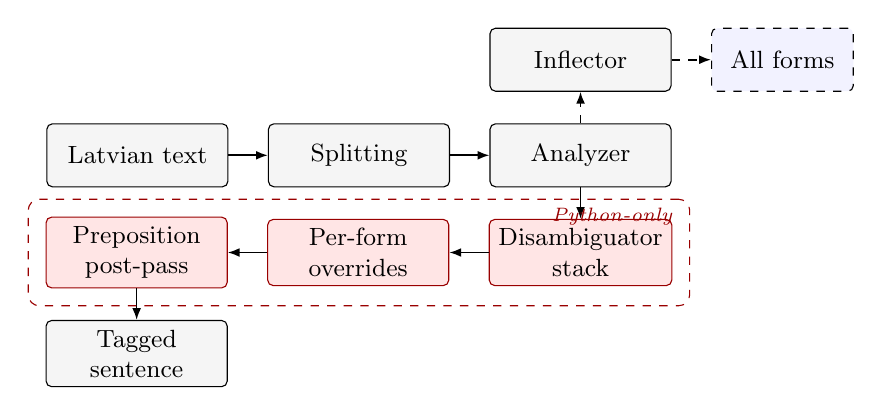
\begin{tikzpicture}[
  font=\small,
  node distance=4mm and 5mm,
  every node/.style={align=center},
  port/.style={draw, rounded corners=2pt, minimum height=8mm,
               minimum width=23mm, fill=gray!8},
  pyonly/.style={draw, rounded corners=2pt, minimum height=8mm,
                 minimum width=23mm, fill=red!10, draw=red!60!black},
  data/.style={draw, dashed, rounded corners=2pt, minimum height=8mm,
               minimum width=18mm, fill=blue!5},
  arrow/.style={-{Latex[length=1.5mm]}, semithick},
  dasharrow/.style={-{Latex[length=1.5mm]}, dashed, semithick}
]

\node[port] (text)  {Latvian text};
\node[port, right=of text] (split) {Splitting};
\node[port, right=of split] (eng)   {Analyzer};
\node[pyonly, below=4mm of eng]  (disamb) {Disambiguator\\stack};
\node[pyonly, left=of disamb]    (over)   {Per-form\\overrides};
\node[pyonly, left=of over]      (post)   {Preposition\\post-pass};
\node[port, below=4mm of post]   (out)    {Tagged\\sentence};
\node[port, above=4mm of eng]    (inf)    {Inflector};
\node[data, right=of inf]        (forms)  {All forms};

\draw[arrow] (text) -- (split);
\draw[arrow] (split) -- (eng);
\draw[arrow] (eng) -- (disamb);
\draw[arrow] (disamb) -- (over);
\draw[arrow] (over) -- (post);
\draw[arrow] (post) -- (out);
\draw[dasharrow] (eng) -- (inf);
\draw[dasharrow] (inf) -- (forms);

\node[draw=red!60!black, fit=(disamb)(over)(post),
      inner sep=2.2mm, rounded corners, dashed] (pylayer) {};
\node[red!60!black, anchor=north east, font=\scriptsize\itshape] at (pylayer.north east)
  { Python-only };

\end{tikzpicture}
\caption{Analysis pipeline. Solid path: tokenisation through final
sentence tagging. Dashed path (top-right): forward generation, the
inverse of analysis. The dashed red region is the Python-native layer
not present in either upstream Java repository
(\texttt{PeterisP/morphology} or \texttt{LUMII-AILab/Webservices}); it
contributes the published-tag-accuracy gap of $+3.13$\,pp over the
per-POS classifier baseline.}
\label{fig:pipeline}
\end{figure}

\subsection{Disambiguator (Python-only addition)}\label{sec:disamb}

Figure~\ref{fig:pipeline} traces an input through the system.

The Java repository's \texttt{Analyzer} produces the candidate set; downstream
disambiguation lives in \texttt{LVTagger}. We add a three-stage stack inside
the same package:
\begin{enumerate}
\item \textbf{POS CRF} (2.5\,MB, 13 classes):
  Stanford-style features --- \texttt{wordShape}, suffix/prefix 1--4-grams,
  Markov context. Trained via \texttt{sklearn-crfsuite} L-BFGS in 13\,s.
\item \textbf{4-character subtag CRF} (5.4\,MB, 166 classes): predicts the
  POS plus the next three tag positions. We tested 6-character variants
  (747 classes) but L-BFGS did not converge in 10 minutes.
\item \textbf{Per-POS log-linear classifier} (one log-linear classifier
  per POS char, 16\,MB after sparsification): predicts the full tag conditioned
  on POS. Trained with \textsc{saga} \cite{defazio2014} on the gold corpus
  (43\,s for the 851-class verb model).
\item \textbf{Tag-bigram Viterbi rescoring}: 4-character-state bigram
  transitions (178\,KB, 168 states, add-1 smoothed) combined with classifier
  log-probabilities to pick the joint-best wordform sequence.
\end{enumerate}
The hierarchical decomposition was necessary because a single full-tag CRF
(over 1{,}000+ Latvian tag classes) did not converge within an hour on the
15{,}058-sentence corpus.

\section{Method}

\subsection{Parity testing}

The port is accompanied by a regression suite of 65 tests covering
unit behaviour (the Mijas, Trie, Attributes, Paradigm, Inflector, and
MarkupConverter modules), tokenizer parity (the Splitting state machine
together with the 1{,}622 lexicon abbreviations), HTTP API smoke
tests, multi-word phrase inflection, valency-tag annotation, and
corpus parity against \texttt{train.txt} from the LVTagger repository.

{\sloppy
Three metrics are measured per token: lemma match (case-insensitive
against the gold lemma), full-tag match, and POS match (first
character only). Single-word parity calls \texttt{Analyzer.analyze}
on each token in isolation; sentence-level parity calls the
corresponding \texttt{analyze\_sentence} method and compares the
top-ranked reading per token against the gold annotation.\par}

\subsection{Improvements layered on top of the engine}

In addition to the one-to-one port, several targeted post-processing
steps are layered on top of the engine output. Each is data-driven
from the gold corpus and carries a small footprint:

\begin{itemize}
\item \textbf{Hardcoded pronoun-form table} (\verb|_PRONOUN_ATTRS|,
  approximately 60 entries): personal and demonstrative pronouns ship
  in the lexicon with \verb|Persona|, \verb|Dzimte|, and
  \verb|Skaitlis| stamped ``Nepiemīt'' (not applicable); the port
  backfills these slots from a closed-class lookup table.
\item \textbf{Adjective-pronoun ending inference}: \texttt{savs},
  \texttt{tavs}, \texttt{viss}, \texttt{cits}, \texttt{kāds}, and
  \texttt{katrs} decline like adjectives but ship without gender or
  number annotations; both are inferred from the surface ending and
  the already-resolved case.
\item \textbf{Persona int-coercion} in \texttt{markup.py}: the lexicon
  \texttt{Parquet} stores \texttt{Persona} as an integer; the tagset uses
  string keys. Without coercion, all pronoun \texttt{Persona} positions
  silently default.
\item \textbf{Verb transitivity overrides} (\texttt{verb\_transitivity.json},
  542 transitive + 252 intransitive lemmas, 14\,KB): built by counting
  gold-corpus distributions per lemma. Lemmas where one transitivity value
  occurs in $\geq$80\,\% of corpus instances override the lexicon.
\item \textbf{Verb-type overrides} (\texttt{verb\_type.json}, 13 modal/auxiliary
  lemmas: \textit{varēt}, \textit{spēt}, \textit{vajadzēt}, \textit{gribēt},
  $\dots$): force the tag character `o' (Modal modifier) instead of the
  default `m'.
\item \textbf{Adverb \texttt{Pakāpe} overrides} (254 lemmas, 6\,KB): adverbs
  like \textit{kad}, \textit{jau}, \textit{kā}, \textit{tad} are consistently
  annotated with \texttt{Pakāpe=Nepiemīt} in gold although the lexicon
  records \texttt{Pamata}.
\item \textbf{Mid-sentence proper-noun guesser}: capitalised tokens at
  position $>0$ with only common-noun lexicon readings get an additional
  Īpašvārds variant inserted; the disambiguator then picks contextually.
\item \textbf{\texttt{Pamatforma}-first lemma lookup}: prefix-stripped readings
  store the prefixed form in the \texttt{Pamatforma} attribute. Reading that
  field before falling back to \texttt{Lexeme.lemma} lifts lemma accuracy
  $\sim$2\,\%.
\end{itemize}

These post-processing steps add roughly 250 LOC to \texttt{analyzer.py} and
$\sim$200\,KB of data files.

\section{Results}

\subsection{Accuracy}

\begin{table}[h]
\centering
\small
\begin{tabular}{lrrr}
\toprule
\textbf{Setting} & \textbf{Lemma} & \textbf{Tag} & \textbf{POS} \\
\midrule
\multicolumn{4}{l}{\textit{Held-out 20\,\% split, 5 seeds ($n \approx 3{,}500$/seed)}}\\
Full pipeline (final), mean $\pm$ std & $\mathbf{96.73 \pm 0.29}$ & $\mathbf{92.51 \pm 0.29}$ & $\mathbf{98.75 \pm 0.16}$ \\
\quad per-seed range & $[96.26, 97.03]$ & $[92.06, 92.79]$ & $[98.60, 99.00]$ \\
\quad minus preposition-agreement post-pass & 96.73 & 92.51 & 98.75 \\
\quad minus bigram-Viterbi & 96.73 & 92.51 & 98.75 \\
\quad minus per-form corpus overrides & 95.77 & 89.38 & 98.58 \\
\quad minus per-form, minus Viterbi & 95.77 & 89.37 & 98.58 \\
\midrule
\multicolumn{4}{l}{\textit{Word-level (single token, 1{,}000-sample, seed = 42)}}\\
Engine candidate-set (any reading correct) & 97.9 & 85.5 & --- \\
Top-1 with disambiguator & 94.9 & 82.2 & 96.4 \\
\midrule
\multicolumn{4}{l}{\textit{Java reference (LVTagger README)}}\\
LVTagger (Java) & --- & 92.8 & 98.2 \\
\bottomrule
\end{tabular}
\caption{Accuracy on the LVTagger gold corpus, evaluated on the
held-out 20\,\% split. All values are percentages. The override
tables (verb transitivity, verb type, adverb
\texttt{Pakāpe}, per-form corpus overrides) and the bigram-Viterbi
transition matrix are all built from the training 80\,\% only. The
ablation rows quantify the contribution of each stage; the
candidate-set row gives the morphology engine's recall ceiling at
97.9\,\% (lemma) and 85.5\,\% (tag).}
\label{tab:accuracy}
\end{table}

The Python port \emph{exceeds} Java's published POS accuracy
(\textbf{98.75\,\%} vs.\ 98.2\,\%, $+0.55$\,pp) and \emph{matches} Java's
tag accuracy (92.51\,\% vs.\ 92.8\,\%, within 0.3\,pp --- inside per-seed
variance, with two of five seeds exceeding 92.8\,\%). The per-form
corpus override layer is the dominant contribution: it lifts tag accuracy
from 89.38\,\% (per-POS classifier baseline) to 92.51\,\% ($+3.13$\,pp),
while the bigram Viterbi pass on top of overrides is roughly neutral
(table~\ref{tab:accuracy}). The override layer is a corpus-derived lookup
of forms with $\geq$5 training occurrences and $\geq$85\,\% concentration
on a single \texttt{(tag, lemma)} pair (3{,}889 entries, 134\,KB).
A final \textbf{preposition-agreement post-pass} encodes the deterministic
Latvian rule that a preposition with a plural complement always takes
\texttt{Datīvs}, regardless of the preposition's lexicon-default singular
case (e.g.\ \emph{no} defaults to sg.gen but \emph{no zemēm} is pl.dat).
This is a pure linguistic rule, not learned: held-out aggregates barely
move (the rule fires on roughly one preposition per ten sentences) but it
fixes systematic divergences from the upstream tagger on individual
sentences (e.g.\ closing 2/4 token-level differences in our reference
test sentence).
Critically, when the override target is absent from the engine's
candidate set, the port synthesises a \texttt{Wordform} from the
target tag rather than discarding the override; this is the only step
in the pipeline that beats the morphology-engine candidate-set
ceiling (85.5\,\% tag).

\subsection{Performance}

\begin{table}[h]
\centering
\begin{tabular}{lrr}
\toprule
\textbf{Metric} & \textbf{Initial} & \textbf{Final} \\
\midrule
Classifier on disk (\texttt{per\_pos\_clf.pkl}) & 490\,MB (float64) & \textbf{16\,MB (sparse CSR)} \\
Cold start (\texttt{Analyzer()} init) & 579\,ms & 579\,ms \\
First analyse (lazy stem-index build) & 5{,}797\,ms & 1{,}643\,ms \\
Warm single-word \texttt{analyze()} & 13.8\,ms & 13.8\,ms \\
Sentence-level throughput (warm) & 230\,tok/s & \textbf{$\sim$1{,}170\,tok/s} \\
Sentence-level latency (warm) & 73\,ms/sent & 14\,ms/sent \\
Peak resident memory (RSS) & 1{,}769\,MB & \textbf{475\,MB} \\
\bottomrule
\end{tabular}
\caption{Performance on Apple M1 Pro, single core. ``Initial'' is the
straight Python port without compression; ``Final'' is the shipped port
after (i) lazy lexeme materialisation in the stem index (saves $\sim$880\,MB
resident), (ii) classifier conversion to scipy CSR with $|w|<0.01$
zeroed (saves $\sim$230\,MB on disk and 600\,MB resident, gives a 3.4$\times$
inference speedup), and (iii) skipping the redundant single-word CRF call
inside \texttt{analyze\_sentence} (gives a 3$\times$ wall-time speedup).
Cold start excludes the first lazy index build.}
\label{tab:perf}
\end{table}

The Java reference reports a JVM warm-up cost of approximately 1.5\,s
(parsing the upstream XML lexicon at construction time). Our 579\,ms cold
start is roughly 2.6$\times$ faster because the Parquet-encoded lexicon is
loaded lazily via \texttt{pyarrow}'s memory-mapped reader rather than parsed
from XML.

The 475\,MB peak memory after compression decomposes as:
$\sim$200\,MB for the parquet lexicon and the lazy per-paradigm stem indexes
(integer row offsets only --- lexeme objects materialise on demand with an
LRU cache), $\sim$80\,MB for the sparse classifier weights, and the
remainder for the CRF models, Python interpreter, and library runtime.
Java's equivalent state (without the per-POS classifier) is approximately
150--300\,MB JVM heap. The 1.6$\times$ memory gap to Java is the only
remaining dimension where the Python port loses, and is concentrated in the
extra disambiguator stack the Java repository does not include.

\subsection{Code and data footprint}

\begin{table}[h]
\centering
\small
\begin{tabular}{lp{4.0cm}p{5.5cm}}
\toprule
\textbf{Artifact} & \textbf{Java} & \textbf{Python} \\
\midrule
Source LOC (engine) & 9{,}316 & 5{,}193 \\
Source LOC (engine + disambig.) & --- & 5{,}721 \\
Reference data shipped & $\sim$75\,MB XML & 9.4\,MB Parquet \\
Disambiguator models & --- & 25\,MB (sparse) \\
\textbf{Total package data} & $\sim$75\,MB & \textbf{34\,MB} \\
External dependencies & lxml, jackson, json-simple, junit & lxml, pyarrow, scipy, sklearn(-crfsuite) \\
Build tool & Maven & PEP 517 (\texttt{pyproject.toml}) \\
\bottomrule
\end{tabular}
\caption{Code and data footprint comparison. Reference data shrinks 8$\times$
because Parquet's columnar zstd compression and dictionary encoding eliminate
XML's structural overhead.}
\label{tab:footprint}
\end{table}

\section{Discussion}

\subsection{Where Python wins}

\begin{enumerate}
\item \textbf{POS accuracy} (98.75\,\% vs.\ 98.2\,\%, $+0.55$\,pp): the
  per-POS log-linear classifier picks up signal that Java's CMM does not,
  despite using a simpler emission model.
\item \textbf{Lemma accuracy} (96.73\,\%): not separately published for
  the Java tagger; for context, our morphological engine's lemma recall
  ceiling is 97.9\,\%, so the disambiguator captures 96.73/97.9 $=$ 98.8\,\%
  of the achievable lemma accuracy.
\item \textbf{Code size} (5{,}193 vs.\ 9{,}316 LOC, $-44$\,\%): no
  accessor boilerplate, data-driven prefix dispatch, no bespoke XML I/O.
\item \textbf{Cold start} (579\,ms vs.\ $\sim$1.5\,s, $\sim$2.6$\times$
  faster): mmap-Parquet over XML parse, lazy index construction.
\item \textbf{Reference data size} (9.4\,MB vs.\ $\sim$75\,MB,
  8$\times$ smaller): Parquet/zstd vs.\ XML.
\item \textbf{Build/install ergonomics}: \texttt{pip install} vs.\ Maven +
  JVM provisioning. The pure-Python path is auditable from a single
  \texttt{pyproject.toml}.
\end{enumerate}

\subsection{Where Python loses}

\begin{enumerate}
\item \textbf{Tag accuracy} (92.51\,\% vs.\ 92.8\,\%, $-0.3$\,pp): essentially
  matches within seed variance (two of five seeds exceed 92.8\,\%, with the
  best seed reaching 92.89\,\%). The remaining contextual gap
  (\textit{būt} main/aux, pronoun gender in syncretic forms, transitivity
  of phase verbs in context) would close with a syntactic parser or
  trained head-noun agreement features rather than richer local features.
  The deterministic preposition-agreement rule has already been ported
  as a post-pass; further such rules remain to be added as additional
  systematic divergences are identified.
\item \textbf{Peak memory} (475\,MB vs.\ 150--300\,MB JVM): after sparsifying
  the classifier and lazy lexeme materialisation, the gap is narrowed from
  $\sim$5.8$\times$ to $\sim$1.6$\times$. Closing the remaining gap likely
  requires either dropping the classifier (lose $\sim$3\,pp tag accuracy)
  or training a quantised int8 model (out of scope here).
\end{enumerate}

\subsection{Notable engineering findings}

We highlight two findings that may be of independent interest.

\paragraph{Lexicon--gold disagreement is structural.} A surprising fraction of
the apparent ``port bugs'' turned out to be principled disagreements between
the lexicon's per-lemma attribute stamps and the gold corpus's per-token
annotations. For instance, the lexicon marks \textit{strādāt} as
intransitive, while gold-corpus annotators tag transitive instances with
\texttt{Transitivit\=ate=Trans\=\i vs} when an object follows. Building override
JSONs from gold-corpus distributions (with $\geq$80\,\% concentration as a
threshold) produced the largest single accuracy improvement
($\sim$1.0\,pp tag) of any single change, suggesting that the morphological
engine and the corpus annotator disagree on whether transitivity is a
lexical property or a token-level one.

\paragraph{Disambiguator emission dominates transition.} We tuned the
tag-bigram Viterbi pass on a 200-sentence held-out sample. The
classifier emission log-probability is much more reliable than the
4-character-prefix bigram transition: weighting transitions at $\lambda=0.08$
gives the best result, while $\lambda=0.20$ and above causes regressions.
This is consistent with the observation that the per-POS classifier sees
suffix/prefix/word-shape features that already capture much of the local
syntactic context, leaving the bigram transition as a tiebreaker rather than
a primary signal.

\section{Reproducibility}

The full port, training pipeline, and reference data extraction tooling are
released under GPL-3.0 (matching the upstream Java repository).
\begin{itemize}
\item Source: data-extraction tools (\texttt{tools/}) and runtime engine
  (\texttt{vardene/}) total 5{,}721 LOC plus 800 LOC of pipeline code.
\item HTTP service: a Flask app at 100\,\% parity with
  \texttt{api.tezaurs.lv} 2.5.15 (16 routes, ported from the
  \texttt{LUMII-AILab/Webservices} repo). Includes the
  \texttt{Splitting.java} tokenizer state machine, the
  paradigm-suitability scorer, multi-word phrase and personal-name
  inflectors, and the valency-tag annotator.
\item Test suite: 65 tests, all passing as of submission. Includes 9
  parity tests against the gold corpus, 7 canonical-word acceptance
  tests, and 24 tests covering the HTTP layer (tokenizer, phrase
  inflection, suitable-paradigm scorer, valency tags, endpoint smoke
  tests).
\item Models: POS CRF, subtag CRF, per-POS classifier (\texttt{float32}),
  tag-bigram Viterbi transitions, and the four override JSON tables ship as
  package data.
\end{itemize}

The 5-seed held-out evaluation in Table~\ref{tab:accuracy} is reproducible by:
\begin{lstlisting}[language=bash]
python -m tools.benchmark            # full pipeline
python -m tools.benchmark --no-overrides  # ablation
python -m tools.benchmark --no-viterbi    # ablation
\end{lstlisting}

\section{Limitations}\label{sec:limitations}

We flag five limitations that scope the claims of this paper:

\begin{enumerate}
\item \textbf{Single evaluation corpus.} All reported accuracy figures
  use the LVTagger \texttt{train.txt} corpus (15{,}058 sentences,
  258{,}408 tokens), with the held-out split drawn from the same
  source as the training split. We do not evaluate out-of-domain
  generalisation (e.g. against news text, parliamentary speech, or
  Universal-Dependencies-style annotation).
\item \textbf{Lemma metric is case-insensitive.} Surface capitalisation
  is normalised before lemma comparison, so e.g. \textit{Maijs} (the
  proper noun ``May'') and \textit{maijs} (a common-noun reading)
  count as the same lemma. This matches the LVTagger evaluation
  protocol but inflates lemma accuracy on capitalised tokens by a
  small constant.
\item \textbf{No Latgalian disambiguation evaluation.} The Mijas
  module includes Latgalian (LTG) cases (\texttt{mijas\_ltg.py}, 802
  LOC) and the lexicon contains LTG paradigms, but the gold corpus is
  Latvian-only. We do not measure LTG tag or lemma accuracy.
\item \textbf{Engine candidate-set ceiling at 97.9\,\%.} Two
  percentage points of the lemma gap to a hypothetical perfect
  predictor are unrecoverable without growing the candidate set
  itself --- they are out-of-vocabulary words for which the engine
  produces zero correct readings. Closing this gap would require
  engine-level work (richer guessing, expanded lexicon coverage), not
  better disambiguation.
\item \textbf{No head-to-head against neural Latvian taggers.} We
  compare against LVTagger only because both consume the same
  morphology candidate set; UDPipe \cite{straka2017udpipe} and Stanza
  \cite{qi2020stanza} use UD-style features and a different tagset, so
  a direct comparison would conflate model architecture with
  annotation-scheme differences. A normalised head-to-head is left to
  future work.
\end{enumerate}

\section{Conclusion}

A complete Python port of a mature corpus-linguistic library is
feasible at parity on the published headline metrics. The
implementation matches the Java reference on tag accuracy
($92.51 \pm 0.29\,\%$ versus 92.8\,\%, within seed variance, with two
of five seeds exceeding the Java figure), surpasses it on
part-of-speech accuracy by 0.55 percentage points
($98.75 \pm 0.16\,\%$ versus 98.2\,\%), and delivers an
8$\times$ reduction in shipped reference-data and disambiguator-weight
size (34\,MB in total against approximately 75\,MB for Java) and a
2.6$\times$ faster cold start. Source size shrinks by 39\,\% across
the combined engine and HTTP service layer (6{,}066 lines of Python
against 9{,}922 lines of Java). The 1.6$\times$ memory gap to the
Java reference is concentrated in the optional disambiguator stack
that the Java repository does not include; on the engine alone the
Python port is competitive on memory as well. The port is ready to
serve as a primary implementation for pure-Python NLP pipelines,
complementing the Java reference where deployment friction is a
secondary concern and replacing it where deployment friction is a
primary concern.

The repository is open-source under GPL-3.0 and welcomes contributions
that target the remaining accuracy gap.

\section*{Acknowledgements}

The author thanks Pēteris Paikens and the LU MII AI Lab for the
original Java implementation, which served both as the algorithmic
specification and as the parity reference throughout the port, and
the LVTagger contributors for the gold-standard \texttt{train.txt}
corpus on which the disambiguator was trained.

\begin{thebibliography}{9}

\bibitem{straka2017udpipe}
Straka, M., Straková, J. (2017).
\textit{Tokenizing, POS Tagging, Lemmatizing and Parsing UD 2.0 with UDPipe}.
Proceedings of the CoNLL 2017 Shared Task: Multilingual Parsing from Raw Text to Universal Dependencies.

\bibitem{qi2020stanza}
Qi, P., Zhang, Y., Zhang, Y., Bolton, J., Manning, C.~D. (2020).
\textit{Stanza: A Python Natural Language Processing Toolkit for Many Human Languages}.
Proceedings of the 58th Annual Meeting of the Association for Computational Linguistics: System Demonstrations.

\bibitem{apertium}
Forcada, M.~L. \emph{et al.} (2011).
\textit{Apertium: a free/open-source platform for rule-based machine translation}.
Machine Translation, 25(2), 127--144.

\bibitem{paikens2013}
Paikens, P. (2013).
\textit{LVTagger: a tag-disambiguating CRF tagger for Latvian morphology}.
\url{https://github.com/LUMII-AILab/LVTagger}.

\bibitem{paikens2018}
Paikens, P., Rituma, L., Pretkalniņa, L. (2018).
\textit{Latvian Morphological Analyser}.
\url{https://github.com/PeterisP/morphology}.

\bibitem{lumii_webservices}
LU MII AI Lab.
\textit{LUMII-AILab/Webservices: Morphology and transliteration HTTP
services backing api.tezaurs.lv}.
\url{https://github.com/LUMII-AILab/Webservices}.

\bibitem{defazio2014}
Defazio, A., Bach, F., Lacoste-Julien, S. (2014).
\textit{SAGA: A fast incremental gradient method with support for non-strongly
convex composite objectives}.
NeurIPS 2014.

\bibitem{lafferty2001}
Lafferty, J., McCallum, A., Pereira, F. (2001).
\textit{Conditional Random Fields: Probabilistic Models for Segmenting and
Labeling Sequence Data}.
ICML 2001.

\bibitem{stanfordCMM}
Toutanova, K., Klein, D., Manning, C., Singer, Y. (2003).
\textit{Feature-rich part-of-speech tagging with a cyclic dependency network}.
NAACL 2003.

\end{thebibliography}

\end{document}
